%- datasets
%-- unimorph
%-- bibles corpus?
%-- celex
%- permute phonemes
%- permute syllables
%- permute phonemes only within syllables
%- permute morphemes 
%\section{Morphology}

The memory--surprisal trade-off described in Section~\ref{sec:ms-tradeoff} applies not only at the level of words, but also at the level of any linguistic element, including morphemes within words. Therefore, just as word orders are influenced by information locality, the order of morphemes within words should be structured so that morphemes which predict each other are close to each other.

Here, we apply the memory--surprisal trade-off to explain the order of morphemes within morphologically complex words in two agglutinative languages. We study two agglutinative languages for which extensive corpora with hand-annotated morphological segmentation and labeling are available: Japanese and Sesotho.


\paragraph{Verb Suffixes in Japanese}

In Japanese, verbs are marked with an extensive number of suffixes. For example, the following verb forms are marked with multiple suffixes:

\ex.\ag. mi  rare mash yoo \\
%Stem (3) (5) (8) \\
see  \textsc{passive}  \textsc{politeness}  \textsc{future} \\
`will be seen'
\bg. mi taku nakat ta \\
%Stem (6) (7) (8) \\
see \textsc{desiderative} \textsc{negation} \textsc{past} \\
`did not wish to see'

Based on corpus data and the linguistic literature on Japanese, we identified the following frequent verb suffixes, occurring in the following order outwards from the verb (see SI for details).


\begin{enumerate}
\item \textit{suru}: obligatory suffix after Sino-Japanese words when they are used as verbs
\item Valence: causative (-\textit{ase}-) (\citet[142]{hasegawa2014japanese}, \citet[Chapter 13]{kaiser2013japanese})
\item Voice: passive (-\textit{are}-, -\textit{rare}-) \cite[152]{hasegawa2014japanese} \cite[Chapter 12]{kaiser2013japanese}
\item Mood: potential (-\textit{e}-, -\textit{are}-, -\textit{rare}-) \cite[398]{kaiser2013japanese}  
\item politeness (-\textit{mas}-) \cite[190]{kaiser2013japanese}.
\item Mood: desiderative (-\textit{ta}-) \cite[238]{kaiser2013japanese}
\item Negation (-\textit{n}-)
\item Tense/Aspect/Mood/Finiteness: past (-\textit{ta}), future/hortative (-\textit{yoo}) \cite[229]{kaiser2013japanese}, nonfiniteness (-\textit{te}) \cite[186]{kaiser2013japanese}
%\item Nonfiniteness: the suffix -\textit{te} derives a nonfinite form .
\end{enumerate}

%In accordance with Bybee's hierarchy, valence is marked closest to the verb, followed by voice.
%Unlike predicted by the hierarchy, tense/aspect markers are not placed closer to the verb than mood/modality markers.






\paragraph{Verb Affixes in Sesotho}
Sesotho (also known as Southern Sotho) is a Southern Bantu language, spoken by 5.6 Million L1 speakers (REF) mainly in Lesotho and South Africa.
Sesotho verbs are marked with both prefixes and suffixes.
Common prefixes include markers for agreement with subjects and objects; object prefixes always follow subject prefixes \ref{ex:oadireka}.
Common suffixes include markers changing valence and voice, and a mood suffix \ref{ex:ophehela}.

\ex.\ag. oa di rek a \\
\textsc{subject.agreement} \textsc{object.agreement} buy \textsc{indicative} \\
`(he) is buying (it)'  \cite[ex (41)]{demuth1992acquisition} \label{ex:oadireka}
\bg. o pheh el a \\
\textsc{subject.agreement} cook \textsc{applicative} \textsc{indicative} \\
`(he) cooks (food) for (him)'  \cite[ex (41)]{demuth1992acquisition}
\label{ex:ophehela}

We identified affix morphemes and their ordering based on the analysis in \cite{demuth1992acquisition}, supplemented with information from grammars of Sesotho \citep{doke1967textbook,guma1971outline}. See SI for details.
We identified the following prefixes:

\begin{enumerate}
    \item Subject agreement: This morpheme encodes agreement with the subject, for person, number, and noun class (the latter only in the 3rd person) \cite[\textsection 395]{doke1967textbook}.
	    The annotation provided by \cite{demuth1992acquisition} distinguishes between ordinary subject agreement prefixes and agreement prefixes used in relative clauses; we distinguish these morpheme types here.
    
    \item Negation \cite[\textsection 429]{doke1967textbook}
    
    \item Tense/aspect marker   \cite[\textsection 400--424]{doke1967textbook}
    
    \item Object agreement or reflexive marker \cite[\textsection 459]{doke1967textbook}. 
    Similar to subject agreement, object agreement denotes person, number, and noun class features of the object.
\end{enumerate}
We identified the following suffixes:
    
\begin{enumerate}
\item Semantic derivation: reversive (e.g., do $\rightarrow$ undo)  \cite[\textsection 345]{doke1967textbook}
\item Valence: Common valence-altering suffixes include causative, neuter/stative, applicative, and reciprocal \cite[\textsection 307--338]{doke1967textbook}. See SI for details on their meanings.
    \item Voice: passive \cite[\textsection 300]{doke1967textbook} 
    \item Tense \cite[\textsection 369]{doke1967textbook}
    \item Mood \cite[\textsection 386--445]{doke1967textbook}
    \item Interrogative and relative markers, appended to verbs in certain interrogative and relative clauses \cite[\textsection 160, 271, 320, 714, 793]{doke1967textbook}.
    %-\textit{ng}.
    %The interrogative marker -\textit{ng} is an enclitized form of the interrogative `what'.
    %The relative marker -\textit{ng} is suffixed to verbs in relative clauses.
\end{enumerate}



%For prefixes, in agreement with Bybee's hierarchy, subject agreement is encoded in a position further away than TAM features.
%For suffixes, relation to Bybee hierarchy: valence closest, then voice, then tense, then mood.


\subsection{Experiment}
\paragraph{Data Selection and Processing}
For Japanese, we drew on Universal Dependencies data.
In the tokenization scheme used for Japanese, most affixes are separated as individual tokens, effectively providing morpheme segmentations.
We used the GSD corpus, Version 2.4, \citep{tanaka2016universal, asahara2018universal}, as it was the only corpus with a training set and freely available word forms.
In the corpus, verb suffixes largely correspond to auxiliaries (with tag \texttt{AUX}); only a few morphemes tagged \texttt{AUX} are not standardly treated as suffixes (see SI), and one frequent suffix (-\textit{te}) is labeled \texttt{SCONJ}.
We selected verb forms by selecting all chains of a verb (tag \texttt{VERB}) followed by any number of auxiliaries (tag \texttt{AUX}) from the training set of the corpus. When the suffix -\textit{te} (tag \texttt{SCONJ}) followed such a chain, we added this.
We labeled suffixes for underlying morphemes with the help of the lemmatization provided for each suffix in the corpus (see SI for details).
We obtained 15,281 verb forms in the training set and 1,048 verb forms in the held-out set.

%We used the annotation provided in the corpus to identify underlying morphemes (see SI).

%In the corpus, each morpheme is annotated with a lemma, indicating a normalized context-independent representation of the morpheme.
%For both verbs and affixes, this lemma annotation abstracts away from most morphophonological and other allomorphic variation, it thus largely identifies underlying morphemes (see SI for limitations).

For Sesotho, we used the Demuth Corpus \citep{demuth1992acquisition} of child and child-directed speech, containing about 13K utterances with 500K morphemes.
The corpus has very extensive manual morphological segmentation and annotation; each verb form is segmented into morphemes, which are annotated for their function.
Sesotho verbs carry both prefixes and suffixes.
We extracted 37K verb forms (see SI for details).
We randomly selected 5\% to serve as held-out data and used the remaining 95\% as training data.


\paragraph{Estimating Memory-Surprisal Tradeoff}
As in many languages, affixes in Japanese and Sesotho show morphophonemic interactions between neighboring morphemes; for instance, the Japanese politeness morpheme -\textit{mas}- takes the form -\textit{masu} when it is word-final, while it has the allomorph -\textit{mase} when followed by the negation suffix -\textit{n}.

To control for these interactions, we model prediction on the level of morphemes sequences.
That is, we represent each verb form as a sequence of a stem and suffix morphemes, abstracting away from morphophonemic interactions.
See SI for results when modeling prediction on the level of phonemes.

We calculate $I_t$ by estimating an $n$-gram model on the training set and then computing cross-entropies $H[X_t|X_{1\dots t-1}]$ on the held-out set using Kneser-Ney smoothing.
The model may overfit as the context size $t$ increases, leading to higher cross-entropies for larger values of $t$.
To mitigate this problem, we estimate
\begin{equation}
H'_t := \min_{s \leq t} H_s    
\end{equation}
ensuring that $H'_t$ can only decrease as the context size $t$ increases.
Similar results are obtained when instead using the simple `naive' estimator for $I_t$ on the training set, see SI.

\paragraph{Parameterizing Alternative Orderings}

We parameterize alternative affix orderings by assigning a weight in $[0,1]$ to each morpheme.
Given such a grammar, affixes are ordered by the values assigned to their underlying morphemes.
We consider all morphemes annotated in the corpora, including low-frequency ones going beyond the ones identified above (see SI for details).



\paragraph{Creating Optimal Orders}

We optimize orderings for the AUC under the memory-surprisal tradeoff curve with an adaptation of the hill climbing method used by (CITE) to optimize word order grammars for the length of syntactic dependencies and trigram surprisal.

We randomly initialize the assignment of weights to morphemes, and then iteratively change the assignment to reduce AUC.
In each iteration, we randomly choose one morpheme, and evaluate AUC for each way of ordering it between two other morphemes.
We then update the weights to the ordering that yields the lowest AUC.

To speed up optimization, we restrict to morphemes occurring at least 10 times in the corpus for 95\% of iterations, and to 10\% of possible orderings in each step.
These choices vastly reduce computation time by reducing time spent on low-frequency morphemes.

This optimization method is approximate, as it only guarantees convergence to a local optimum, not to a globally optimal assignment.

We ran this method for 1,000 iterations. Empirically, AUC converges after a few hundred iterations.
We ran the algorithm ten times and selected the five runs with the lowest AUC values, i.e., those where optimization was most successful.

\subsection{Results}

In Figure~\ref{fig:jap-phon-morph}, we compare the area under curve of the memory-surprisal tradeoff for Japanese and Sesotho under different orderings.
Both observed orders and the aproximately optimized grammars show lower AUCs than all random baseline samples.
For comparison, we also show AUC for the order resulting from \emph{reversing} all suffix chains in the observed orders; this results in high AUC even exceeding most random grammars.
These results show that Japanese and Sesotho affix orderings enable approximately optimal memory-surprisal tradeoffs.

%\begin{figure}
%	\begin{center}
%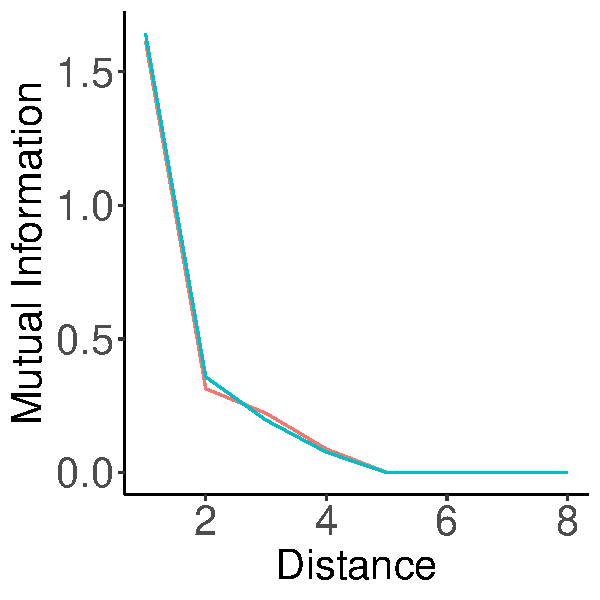
\includegraphics[width=0.3\textwidth]{figures/Japanese-suffixes-byPhonemes-it-heldout.pdf}
%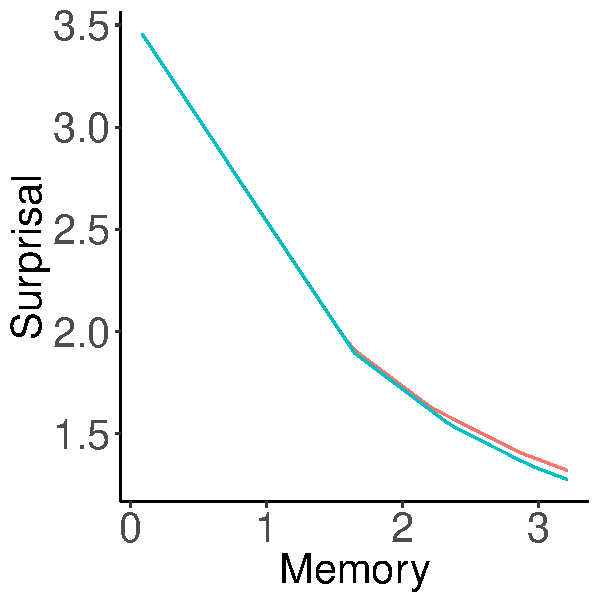
\includegraphics[width=0.3\textwidth]{figures/Japanese-suffixes-byPhonemes-memsurp-heldout.pdf}
%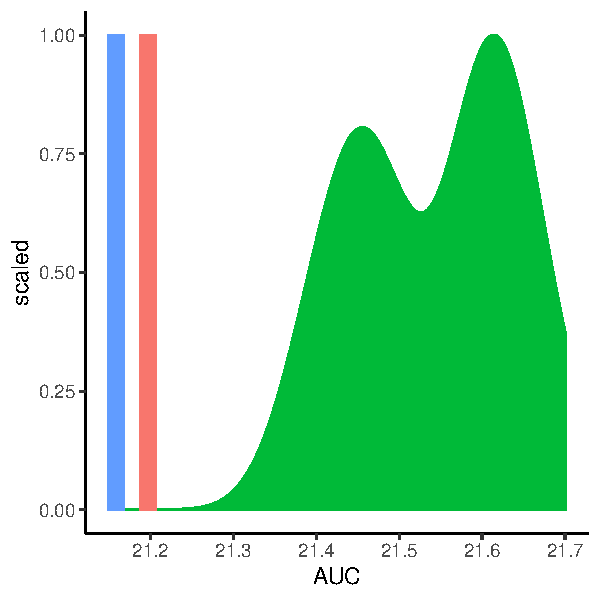
\includegraphics[width=0.3\textwidth]{figures/Japanese-suffixes-byPhonemes-auc-hist-heldout.pdf}
%
%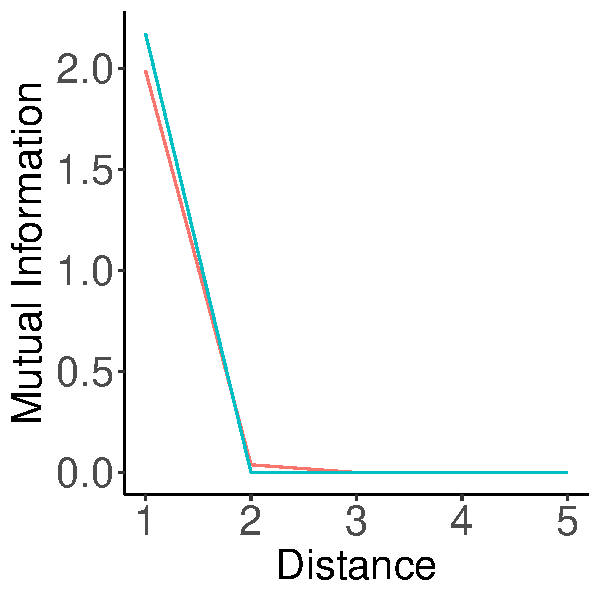
\includegraphics[width=0.3\textwidth]{figures/Japanese-suffixes-byMorphemes-it-heldout.pdf}
%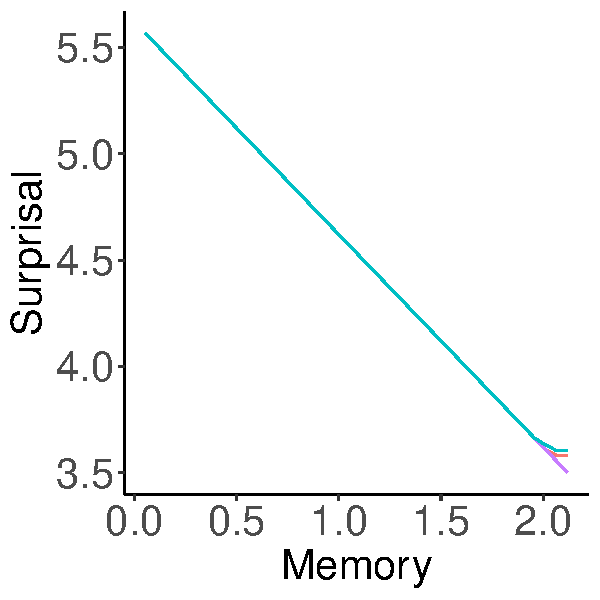
\includegraphics[width=0.3\textwidth]{figures/Japanese-suffixes-byMorphemes-memsurp-heldout.pdf}
%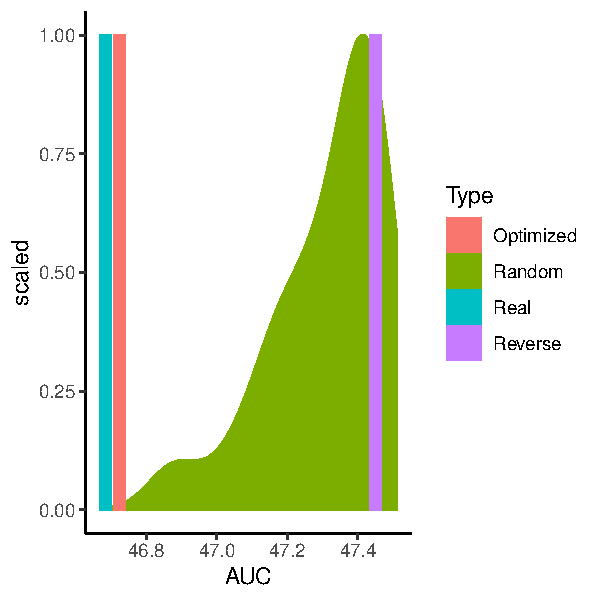
\includegraphics[width=0.3\textwidth]{figures/Japanese-suffixes-byMorphemes-auc-hist-heldout.pdf}
%\end{center}
%	\caption{Areas under the memory-surprisal tradeoff curve for Japanese verb suffixes.}\label{fig:jap-phon-morph}
	%\caption{Japanese verb suffixes, measuring prediction on the level of phonemes (top) and morphemes (bottom), for real (blue), random (green), and approximately optimized (red) orderings. Left: $I_t$ as a function of $t$. Center: Memory-surprisal tradeoff. Right: Areas under the curve for the memory-surprisal tradeoff.}\label{fig:jap-phon-morph}
%\end{figure}


We now ask to what extent the observed morpheme ordering is predicted correctly by approximately optimized grammars.

In Figure~\ref{fig:morph-acc}, we show the accuracy of optimized grammars in predicting affix order in the corpus, together with random baseline figures.
We evaluate accuracy using two methods:
In one method (`Pairs'), we consider, for each verb form in the corpus, all pairs of prefixes (or suffixes).
We then evaluate for what fraction of these pairs, across the corpus, the relative order of the two affixes is as predicted by the grammar.
In the other method, (`Full'), we count what fraction of verb forms in the corpus has exactly the affix ordering predicted by the grammar.


In Japanese, by both measures, optimized grammars recover the observed orders with very high accuracy.
For each grammar, we extracted the ten most common pairs of morphemes whose relative order is incorrectly predicted.
The most frequent divergence is that desiderative and negation are consistently ordered incorrectly; this affects 13 corpus examples.
A few of the optimized grammars show additional divergences among high-frequency morphemes, for instance, some grammars order politeness and negation incorrectly. 
We compare the real grammar with the approximately optimized grammar that achieved the lowest AUC value in Figure~\ref{fig:grammar-table-jap}.

\begin{figure}
    \centering
    \begin{tabular}{llllllll}
	    &	    Real & Optimized \\ \hline\hline
	    &    Stem & Stem \\ \hline
	    1 & suru & suru \\
	    2 & causative & causative \\
	    3 & passive/potential & passive/potential \\
	    4 & desiderative & politeness \\
	    5 & politeness & negation \\
	    6 &negation & desiderative \\
	    7 & future & nonfinite \\
	    & past & past \\
	     & nonfinite & future \\ \hline
    \end{tabular}
    \caption{Comparing order of Japanese affixes in the observed orders (left) and according to an approximatively optimized grammar (right).}
    \label{fig:grammar-table-jap}
\end{figure}



\begin{figure}
    \centering
    \begin{tabular}{llllllll}
	    &	    Real & Optimized \\ \hline\hline
	    1 & Subject & Subject \\
	      & Subject (rel.) & Subject (rel.) \\
	    2 & Negation & Tense/aspect \\
	    3& Tense/aspect & Negation \\
	    4 &Object & Object \\ \hline
	    &Stem & Stem  \\ \hline
	    1 & Reversive & Passive \\
	    2& Causative & Reciprocal \\
	    &Neuter & Tense/aspect \\
	    &Applicative & Neuter \\
	    &Reciprocal & Relative \\
	    3&Passive & Causative \\
	    4&Tense/aspect & Applicative \\
	    5&Mood & Interrogative \\
	    6&Interrogative & Reversive \\
	    &Relative & Mood \\ \hline
    \end{tabular}
	\caption{Comparing order of Sesotho affixes in the observed orders (left) and according to an approximatively optimized grammar (right). Note that order was separately optimized for prefixes and suffixes.}
    \label{fig:grammar-table-sesotho}
\end{figure}


%\begin{figure}
%\begin{center}
%\begin{tabular}{c||llll}
%             &       Pairs & Full \\ \hline\hline
%Optimized for Phoneme Prediction   &   0.962 (SD 0.001) & 0.957 (SD 0.002) \\
%Optimized  &   0.954 (SD 0.009) & 0.945 (SD 0.012) \\ 
%Random Baseline    &  0.504 (SD 0.0) & 0.414 (SD 0.0) \\ 
%\end{tabular}
%\end{center}
%\caption{Accuracy of approximately optimized orderings, and of random baseline orderings, in predicting verb suffix order in Japanese. `Pairs' denotes the rate of pairs of morphemes that are ordered correctly, and `Full' denotes the rate of verb forms where order is predicted entirely correctly. We show means and standard deviations over different runs of the optimization algorithm (`Optimized'), and over different random orderings (`Random').}\label{fig:acc-japanese}
%\end{figure}




\begin{figure}
	\begin{center}
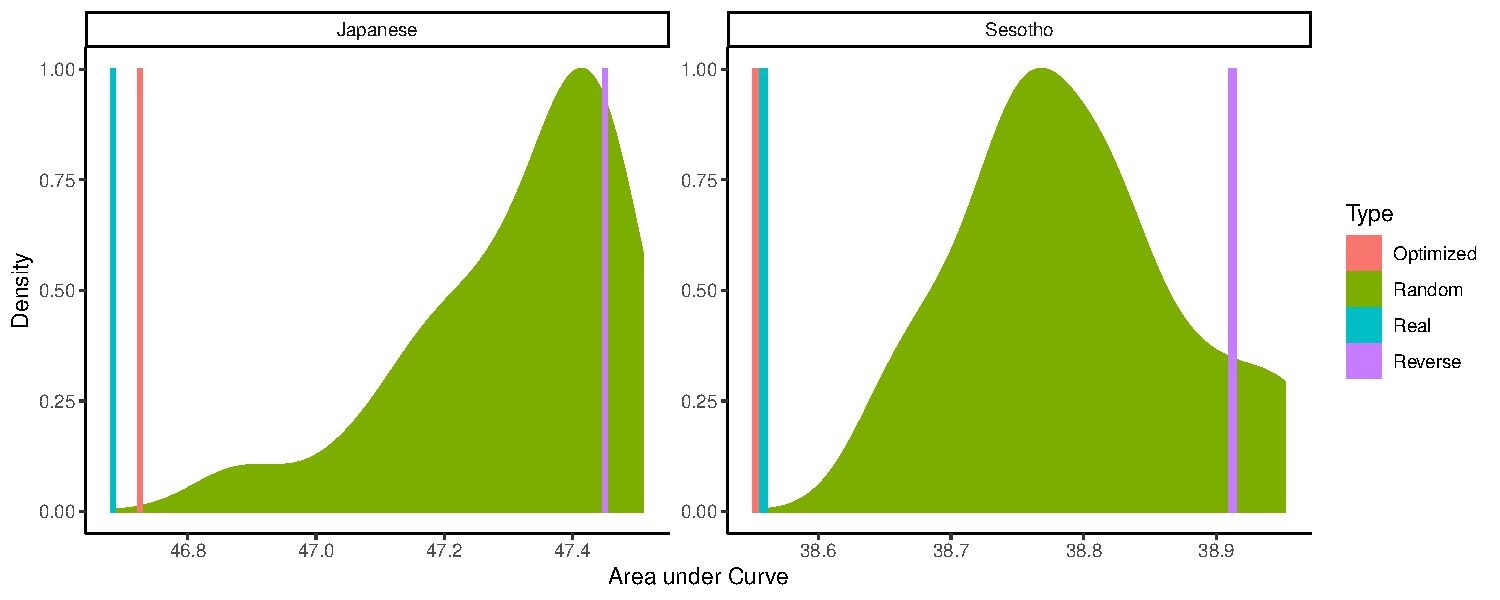
\includegraphics[width=\textwidth]{figures/Both-suffixes-byMorphemes-auc-hist-heldout.pdf}
\end{center}
	\caption{Areas under the curve for the memory-surprisal tradeoff for verb affixes in Japanese (left) and Sesotho (right).}\label{fig:morph-auc}
\end{figure}




In Sesotho, for prefixes, all optimized grammars almost exactly recover the ordering described above.
The only divergence among the high-frequency morphemes is that negation and the tense/aspect prefix are ordered incorrectly; this accounts for only 11 occurrences in the data set, as the two prefixes only rare co-occur
Other divergences affect lower-frequency morphemes.
For suffixes, order is recovered at above-chance accuracies, though with some divergences.
For instance, relative and interrogative suffixes are consistently placed closer to the verb stem than the mood suffix.
Furthermore, valence-changing suffixes are ordered farther away from the stem than various other suffixes, in contrast with the actual orders.
We compare the real grammar with the approximately optimized grammar that achieved the lowest AUC value in Figure~\ref{fig:grammar-table-sesotho}.

\begin{figure}
\begin{tabular}{cc||ll|ll}
             &              & \multicolumn{2}{c}{Prefixes}    & \multicolumn{2}{|c}{Suffixes} \\
             &              & Pairs & Full & Pairs & Full \\ \hline\hline
Japanese & Optimized  & -- &  -- &   0.954 (SD 0.009) & 0.945 (SD 0.012) \\ 
& Baseline    & -- & -- & 0.504 (SD 0.0) & 0.414 (SD 0.0) \\ \hline
%Phon.   &   Optimized  &  0.993 (SD 0.0) & 0.989 (SD 0.0) & 0.792 (SD 0.102) & 0.734 (SD 0.13) \\
%	& Random  &  0.322 (SD 0.253) & 0.195 (SD 0.24) & 0.588 (SD 0.155) & 0.554 (SD 0.167) \\ \hline
Sesotho &   Optimized  &  0.988 (SD 0.0) & 0.989 (SD 0.0) & 0.756 (SD 0.014) & 0.676 (SD 0.017) \\
&   Baseline  &  0.672 (SD 0.305) & 0.604 (SD 0.338) & 0.423 (SD 0.204) & 0.332 (SD 0.211) \\ 
\end{tabular}
\caption{Accuracy of approximately optimized orderings, and of random baseline orderings, in predicting verb affix order in Sesotho. `Pairs' denotes the rate of pairs of morphemes that are ordered correctly, and `Full' denotes the rate of verb forms where order is predicted entirely correctly. We show means and standard deviations over different runs of the optimization algorithm (`Optimized'), and over different random orderings (`Random').}\label{fig:morph-acc}
\end{figure}

\subsection{Discussion}
We have found that the ordering of verb affixes in Japanese and Sesotho provides approximately optimal memory-surprisal tradeoffs.
We further found that many aspects of these languages' ordering rules can be derived from optimizing order for efficient tradeoffs.

Bybee 1985:

verb-valence-voice-aspect-tense-mood-modality-subj.person-subj.number


